\chapter{Lecture 32 - Laplace Equation in Cylindrical Coordinates}
\label{ch:lec32}
\section{Objectives}
\begin{itemize}
\item Solve the steady-state heat equation (Laplace Equation) in cylindrical coordinates for two cases.
\item Re-introduce modified Bessel functions of the first and second kind.
\end{itemize}
\setcounter{lstannotation}{0}

\section{Steady-State Temperature in a Circular Cylinder - Case I}
Consider the boundary value problem below based on the steady-state heat equation in cylindrical coordinates. A schematic of the problem is shown in Figure \ref{fig:lec32-ex1-schematic}.
\begin{table}[h]
\begin{tabular}{l l}
$\substack{\text{Governing} \\\text{Equation}}: $& $\frac{\partial^2 u}{\partial r^2} + \frac{1}{r}\frac{\partial u}{\partial r} + \frac{\partial^2 u}{\partial z^2} + \frac{1}{r^2}\frac{\partial^2 u}{\partial \theta^2}= 0, \ \ \substack{0<r<2, \ \ 0<z<4 \\ \\ 0<\theta<2 \pi}$\\
& \\
$\substack{\text{Boundary} \\ \text{Conditions}}: $ & $u(r,0) = 0, \ u(r,4) = u_0, \ u(2,z) = 0$  \\ 
\end{tabular}
\end{table} 
\begin{marginfigure}
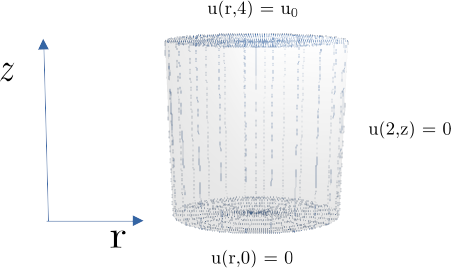
\includegraphics{lec32-ex1-schematic.png}
\caption{Schematic of Case I}
\label{fig:lec32-ex1-schematic}
\end{marginfigure}

\vspace{0.25cm}

\noindent Based on the boundary conditions provided for the problem---none of which are dependent on $\theta$---we can expect that the solution also will be independent of $\theta$ and so the governing equation can be simplified to:
\begin{equation*}
\frac{\partial^2 u}{\partial r^2} + \frac{1}{r}\frac{\partial u}{\partial r} + \frac{\partial^2 u}{\partial z^2} = 0
\end{equation*}

\newthought{As is becoming the usual}, we will solve this problem using separation of variables.

\vspace{0.25cm}

\noindent\textbf{Step \#1:} Assume a product solution:
\begin{equation*}
u(r,z) = F(r)G(z)
\end{equation*}

\vspace{5.0cm}

\noindent\textbf{Step \#2:} Insert the product solution into the governing equation.

\begin{align*}
\frac{\partial^2}{\partial r^2}\left(F(r)G(z) \right) + \frac{1}{r}\frac{\partial}{\partial r}\left(F(r) G(z)\right) + \frac{\partial^2}{\partial z^2}\left( F(r)G(z)\right) &= 0 \\
F_{rr}G + \frac{1}{r}F_rG + FG_{zz} &= 0
\end{align*}

\vspace{0.25cm}

\noindent\textbf{Step \#3:} Separate the variables.

\begin{align*}
\frac{F_{rr}G}{FG} + \frac{1}{r}\frac{F_r G}{FG} + \frac{FG_{zz}}{FG} &= 0 \\
\frac{F_{rr}}{F} + \frac{1}{r}\frac{F_r}{F} + \frac{G_{zz}}{G} &= 0 \\
\frac{F_{rr}}{F} + \frac{1}{r}\frac{F_r}{F} = -\frac{G_{zz}}{G} &= -\lambda
\end{align*}
So the separated equations are:\marginnote{Again, here we multiply the equation for $F(r)$ by $r^2$ to render the equation into a familiar form.}
\begin{align*}
r^2F_{rr} + rF_r + \lambda r^2 F &= 0 \\
G_{zz} - \lambda G &= 0
\end{align*}

\noindent\textbf{Step \#4:} Apply boundary conditions to determine non-trivial product solution(s):

\vspace{0.25cm}

\noindent In the $z$-direction we have only one homogeneous boundary condition whereas in the $r$-direction, the only boundary condition we have is homogeneous.  Therefore we should analyze the equation of $F(r)$ to determine values of $\lambda$ that will admit non-trivial solutions.

\vspace{0.25cm}

\noindent\underline{$\lambda = 0$}:

\vspace{0.25cm}

\noindent In this case the boundary value problem for $F(r)$ is a Cauchy-Euler equation:\marginnote{Reminder: for Cauchy-Euler equations we assume the solution is of the form $F(r)=r^m$.  In this case where the resulting auxiliary equation has a double-root---$m=0,0$---the first solution is a constant ($c_1$) and the second solution is a constant times $\ln r$ so that it is linearly independent.}
\begin{align*}
r^2F_{rr} + rF_r &= 0 \\
r^2[m(m-1)r^{m-2}] + rmr^{m-1} &= 0 \\
r^m[m(m-1) + m] &= 0 \Rightarrow m^2 = 0\\
\Rightarrow F(r) &= c_1 + c_2 \ln r
\end{align*}
We must set $c_2=0$ so that $F(r)$ will remain bounded as $r \to 0$.  Since $u(2,z)=0$, we must stipulate that $F(2)=c_1=0$ so that only the trivial solution will satisfy the boundary conditions if $\lambda = 0$.

\vspace{0.25cm}

\noindent\underline{$\lambda < 0$} where $\lambda = -\alpha^2, \ \alpha>0$

\noindent In this case the boundary value problem for $F(r)$ is:
\begin{equation*}
r^2F_{rr} + rF_r -\alpha^2r^2F = 0
\end{equation*} 
Which we recognize as the parametric modified Bessel's equation of order zero.  The general solution is:\marginnote[-1.5cm]{Reminder: the parametric modified Bessel's equation is of the form:
\begin{equation*}
r^2 F_{rr} + rF_r - (\alpha^2 r^2 + \nu^2)F = 0
\end{equation*}
where $\nu$ is the order of the equation.
}
\begin{equation*}
F(r) = c_1I_0(\alpha r) + c_2 K_0(\alpha r)
\end{equation*}
In case one is not familiar with modified Bessel functions of the first and second kind of order zero---$I_0(r)$ and $K_0(r)$,respectively---the reader might be relieved to be informed that MATLAB has built-in functions available: \lstinline[style=myMatlab]{besseli()} and \lstinline[style=myMatlab]{besselk()}. A plot of these functions is shown in Figure \ref{fig:lec32-mbfs}.
\begin{marginfigure}
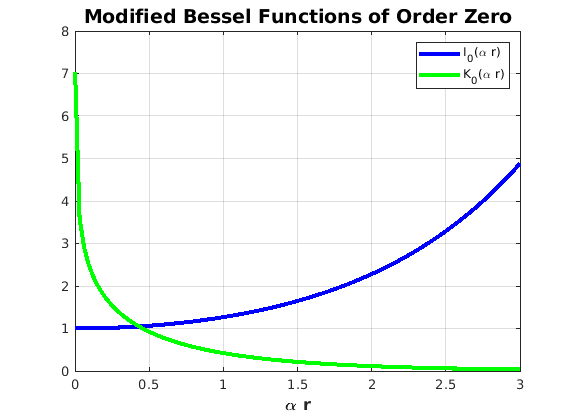
\includegraphics{lec32-mbfs.png}
\caption{Plots of $I_0(\alpha r)$ and $K_0(\alpha r)$ for $\alpha r > 0$.}
\label{fig:lec32-mbfs}
\end{marginfigure}
The salient facts about these functions is that $K_0(\alpha r)$ diverges to infinity as $r \to 0$ and that $I_0(\alpha r)$ is strictly positive for $\alpha r > 0$.  Thus $c_1 = c_2 = 0$ and only the trivial solution satisfies the boundary conditions in the case $\lambda < 0 $.

\vspace{0.25cm}

\noindent\underline{$\lambda > 0 $} where $\lambda = \alpha^2, \ \alpha>0$.

\noindent In this case the boundary value problem for $F(r)$ is:
\begin{equation*}
r^2F_{rr}+rF_r+\alpha^2r^2F = 0
\end{equation*}
Which we recognize as the parametric Bessel's equation of order zero.  The general solution is:
\begin{equation*}
F(r) = c_1J_0(\alpha r) + c_2 Y_0(\alpha r)
\end{equation*}
Since $Y_0(\alpha r)$ diverges to negative infinity as $r \to 0$, we must set $c_2 = 0$.  In order to satisfy the boundary condition at $r=2$:\marginnote[1.5cm]{Use the MATLAB function \lstinline[style=myMatlab]{besselzero()} to get the roots to $J_0(\alpha r)$}
\begin{align*}
F(2) = c_1J_0(2 \alpha) &= 0 \\
\Rightarrow \alpha_n &= \frac{k_{0,n}}{2}
\end{align*}
where we have, on the fly, adopted the notation $\alpha_n$---the $n$\textsuperscript{th} eigenvalue---and $k_{0,n}$ as the $n$\textsuperscript{th} root of the Bessel Function of the first kind of order zero.

\vspace{0.25cm}

\noindent For $\lambda = \alpha^2$, the boundary value problem in the $z$-direction is:
\begin{equation*}
G_{zz}-\alpha^2G = 0
\end{equation*}
Where the general solution is:
\begin{equation*}
G(z) = c_3\cosh{\alpha z} + c_4\sinh{\alpha z}
\end{equation*}
Applying the homogeneous boundary condition at $z=0$ we get:
\begin{align*}
G(0) = c_3 \cancelto{1}{\cosh{0}} + c_4 \cancelto{1}{\sinh{0}} &= 0 \\
= c_3(1) + c_4(0) &= 0 \\
\Rightarrow c_3 &= 0
\end{align*}
The solution in the $z$-direction is, therefore:
\begin{equation*}
G(z) = c_4 \sinh{\alpha_n z}
\end{equation*}

\vspace{0.25cm}

\noindent After combining constants, as usual, the full product solution is:

\begin{equation}
u(r,z) = \sum\limits_{n=1}^{\infty} a_n J_0(\alpha_n r) \sinh{\alpha_n z}
\label{eq:lec32-ex1-sol}
\end{equation}
where $\alpha_n = \sfrac{k_{0,n}}{2}$.

\vspace{0.25cm}

\noindent\textbf{Step \#5:} Apply the remaining boundary condition to determine unknown coefficients.

\vspace{0.25cm}

\noindent The boundary condition that we have not yet used is the non-homogeneous condition applied at the top of the cylinder: $u(r,4) = u_0$.  We must find suitable values of $a_n$ for $n=1,2,3,\dots$ such that:
\begin{equation*}
u(r,4) = \sum\limits_{n=1}^{\infty}a_n J_0(\alpha_n r) \sinh{4\alpha_n} = u_0
\end{equation*}
Once again we have an infinite linear combinations of eigenfunctions on the left and on the right we have a given function---in this case a constant, $u_0$.  We want them to be equal; our job is to determine $a_n$ such that they are equal.  How do we do this?  We multiply both sides by our orthogonal function, and weight function, and integrate.  The resulting equation for $a_n$ is given in Equation \ref{eq:lec32-ex1-coeff}.\marginnote[0.75cm]{Do not forget to include the constant $\sinh{4 \alpha_n}$; it is easy to leave off when you are in a hurry.}
\begin{equation}
a_n = \frac{u_0\int_0^2 J_0(\alpha_n r)r \ dr}{\sinh{4 \alpha_n}\int_0^2 J_0(\alpha_nr)^2 r \ dr}
\label{eq:lec32-ex1-coeff}
\end{equation}
We can create a MATLAB script to construct an approximate solution for a specified value of $u_0$ and a finite number of eigenmodes.  The code for $u_0 = 5$ and $N = 25$ is shown in the listing below.
\marginnote[3.25cm]{
\ref{lst:ann32-1-1} Recall that the first argument to \lstinline[style=myMatlab]{besselzero()} is the order of the Bessel function, the second argument is the number of desired roots, and the third argument is the \emph{kind} of Bessel function---first or second.
}
\begin{lstlisting}[name=lec32-ex1, style=myMatlab]
clear
clc
close 'all'

%% Parameters
R = 2; Z = 4;
Uo = 5; % given temperature on top surface of the cylinder
N = 25;
k = besselzero(0,N,1); % get first n zeros of Jo    /*!\annotation{lst:ann32-1-1}!*/
alpha = k/R;

%% Construct Solution
A = nan(N,1);
u = @(r,z) 0; % initialize the series
for n = 1:N
    A(n) = (Uo/(sinh(Z*alpha(n)))).*...
        integral(@(r) besselj(0,alpha(n)*r).*r,0,R)./...
        integral(@(r) besselj(0,alpha(n)*r).*...
        besselj(0,alpha(n)*r).*r,0,R);
    
    % update the series with the next term
    u = @(r,z) u(r,z) + ...
        A(n)*besselj(0,alpha(n)*r).*sinh(z*alpha(n));    
end


%% Plot results
Rv = linspace(0,R,100);
Zv = linspace(0,Z,200);

[RR,ZZ] = meshgrid(Rv,Zv);
UU = u(RR,ZZ);

figure(1)
surf(Rv,Zv,UU,'edgecolor','none');
title('Laplacian in a Cylinder: Case 1',...
    'fontsize',18,'fontweight','bold');
xlabel('R','fontsize',16,'fontweight','bold');
ylabel('Z','fontsize',16,'fontweight','bold');
zlabel('U','fontsize',16,'fontweight','bold');
view([65 10]);  /*!\annotation{lst:ann32-1-2}!*/
\end{lstlisting}
A cross-section of the temperature distribution is shown in Figure \ref{fig:lec32-ex1-plot-n25}. \marginnote[-3.0cm]{
\ref{lst:ann23-1-2} The \lstinline[style=myMatlab]{view()} function allows you to rotate the plotted image.  It is best to experiment a bit with different arguments to find a view that best presents the results.
}
\begin{marginfigure}
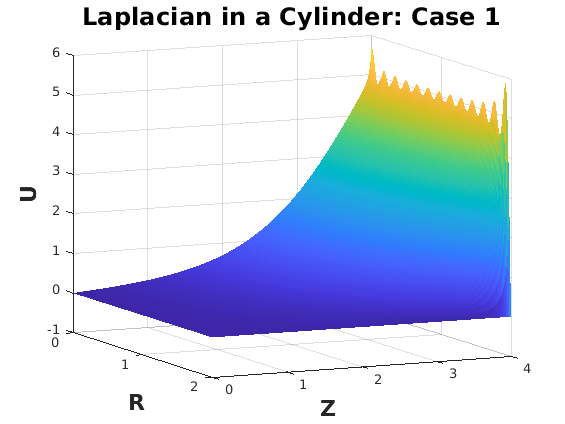
\includegraphics{lec32-ex1-plot-n25.png}
\caption{Cross section of Case I solution for N=25.}
\label{fig:lec32-ex1-plot-n25}
\end{marginfigure}
\newthought{As we have come} to expect, the approximate solution has a certain amount of ``wiggliness'' at points of discontinuity.  In this case, the issue is along the outer rim of the top of the cylinder; on the top of the cylinder, the solution is constant at $u_0 = 5$; on the outer surface of the cylinder the solution is fixed at $u = 0$.  Along the outer rim of the top is where these conflicting solutions come together and the ``wiggliness'' is the result.  If we increase the number of eigenmodes.  A plot with $N=100$ eigenmodes is shown in Figure \ref{fig:lec32-ex1-plot-n100}
\begin{marginfigure}
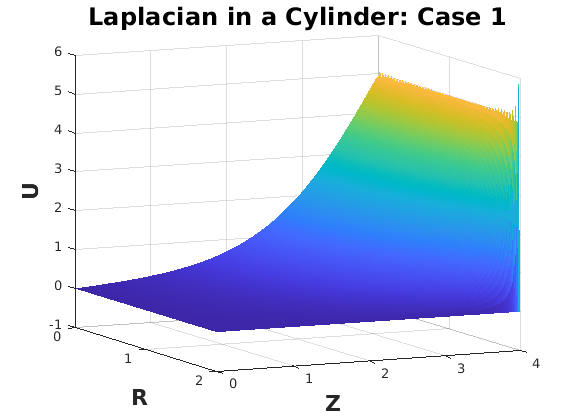
\includegraphics{lec32-ex1-plot-n100.png}
\caption{Cross section of Case I solution for N=100.}
\label{fig:lec32-ex1-plot-n100}
\end{marginfigure}

\section{Steady-State Temperature in a Circular Cylinder - Case II}
Consider another boundary value problem similar to the first except, in this case, there are homogeneous boundary conditions on the top and bottom while the side of the cylinder is maintained at a prescribed temperature.  A schematic is shown in Figure \ref{fig:lec32-ex2-schematic}
\begin{table}[h]
\begin{tabular}{l l}
$\substack{\text{Governing} \\\text{Equation}}: $& $\frac{\partial^2 u}{\partial r^2} + \frac{1}{r}\frac{\partial u}{\partial r} + \frac{\partial^2 u}{\partial z^2} + \frac{1}{r^2}\frac{\partial^2 u}{\partial \theta^2}= 0, \ \ \substack{0<r<1, \ \ 0<z<1 \\ \\ 0<\theta<2 \pi}$\\
& \\
$\substack{\text{Boundary} \\ \text{Conditions}}: $ & $u(r,0) = 0, \ u(r,1) = 0, \ u(1,z) = 1-z$  \\ 
\end{tabular}
\end{table} 
\begin{marginfigure}
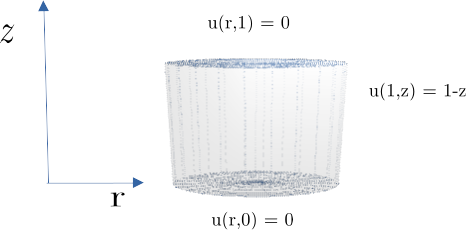
\includegraphics{lec32-ex2-schematic.png}
\caption{Schematic of domain and boundary conditions for Case I.}
\label{fig:lec32-ex2-schematic}
\end{marginfigure}
As with Case I, the boundary conditions are all independent of $\theta$ so we expect the solution to be independent of $\theta$ also, and we can simplify the governing equation to:
\begin{equation*}
\frac{\partial^2 u}{\partial r^2} + \frac{1}{r}\frac{\partial u}{\partial r} + \frac{\partial^2 u}{\partial z^2} = 0
\end{equation*}

\newthought{The details of} Steps \#1 through \#3 of separation of variables are exactly the same for this case; the separated equations are again:
\begin{align*}
r^2F_{rr} + rF_r + \lambda r^2 F &= 0 \\
G_{zz} - \lambda G &= 0
\end{align*}
What makes this case different is the boundary conditions.  Specifically, in the $r$-direction we no longer have a homogeneous boundary condition but in the $z$-direction, we do; therefore we will use the equation for $G(z)$ to determine values of $\lambda$ that admit non-trivial solutions.

\vspace{0.25cm}

\noindent\textbf{Step \#4:} Apply boundary conditions to determine non-trivial product solution(s).

\vspace{0.25cm}

\noindent We have seen this combination of boundary value problem and boundary conditions numerous times before.  $G_{zz}-\lambda G = 0$ and $G(0)=G(1)=0$.  If $\lambda=0$ we know the solution is linear, but the only line that is zero at both ends is $G(z)=0$ so we can discard that case quickly.  If $\lambda > 0$, or $\lambda = \alpha^2, \ \alpha>0$, then we have 
\begin{equation*}
G_{zz} - \alpha^2 G = 0
\end{equation*}
with general solution: $G(z) = c_1 \cosh{\alpha z} + c_2 \sinh{\alpha z}$.  The condition $G(0) = 0$ implies that $c_1 = 0$. The condition $G(1) = 0$ means that $c_2 \sinh{\alpha} = 0$ but, as we have seen before, $\sinh{\alpha}$ is never zero for $\alpha > 0$.  Thus we have no choice but to also set $c_2 = 0$.  

Consequently, our only remaining option is $\lambda < 0$, where we set $\lambda = -\alpha^2, \ \alpha > 0$.  This gives us:
\begin{equation*}
G_{zz} + \alpha^2 G = 0
\end{equation*}
with general solution: $G(z) = c_1 \cos{\alpha z} + c_2 \sin{\alpha z}$.

When we apply the boundary conditions we get:
\begin{align*}
G(z) &= c_1 \cos{\alpha z} + c_2 \sin{\alpha z} \\
G(0) &= c_1 (1) + c_2 (0) = 0 \\
\Rightarrow c_1 &= 0 \\ 
G(1) &= c_2 \sin{\alpha} = 0
\end{align*}
The last condition can be satisfied if $\alpha_n = n \pi$ with $n$ a positive integer.  

\vspace{0.25cm}

\noindent With $\lambda = -\alpha^2$, the equation for $F(r)$ is:
\begin{equation*}
r^2F_{rr}+rF_r - \alpha^2r^2F = 0
\end{equation*}
We recognize this as the parametric modified Bessel's equation of order zero.  The general solution is: $F(r) = c_3I_0(\alpha r) + c_4 K_0(\alpha r)$.  This is fresh in our mind, so we immediately conclude that $c_4 = 0$ since $K_0(\alpha r)$ diverges as $r \to 0$.  The product solutions for this problem are, therefore:
\begin{equation}
u(r,z) = \sum\limits_{n=1}^{\infty} c_n I_0(n \pi r) \sin{n \pi z}
\label{eq:lec32-ex2-sol}
\end{equation}

\vspace{0.25cm}

\noindent\textbf{Step \#5:} Apply the remaining boundary condition to determine the unknown coefficients.

\vspace{0.25cm}

\noindent The boundary condition that we have not yet used is the non-homogeneous condition applied on the outer surface of the cylinder: $u(1,z) = 1-z$.  We must find suitable values of $c_n$ such that:

\begin{equation*}
u(1,z) = \sum\limits_{n=1}^{\infty} c_n I_0(n \pi)\sin{n \pi z} = 1-z
\end{equation*}
Here again, of course, we need to multiply both sides by an orthogonal function (and weight function) and integrate.  In this case, however, the orthogonal set of functions is $\sin{n\pi z}$ and the weight function is $p(z)=1$.\marginnote[-1.0cm]{Students sometimes struggle with this.  The key is to realize that $I_0(n \pi)$ is not really a function but a constant---albeit a tricky one to evaluate.}  Carrying out this (by now routine) task, we obtain the expression for $c_n$ as:
\begin{equation}
c_n = \frac{\int_0^1 (1-z)\sin{n \pi z} \ dz}{I_0(n \pi) \int_0^1 \sin{(n \pi z)}^2 \ dz}
\label{eq:lec32-ex2-coeff}
\end{equation}
In summary, for Case II, the solution is given by Equation \ref{eq:lec32-ex2-sol} with the coefficients given by Equation \ref{eq:lec32-ex2-coeff}.  A plot of the solution for N=150 is given in Figure \ref{fig:lec32-ex2-plot-n150}
\begin{marginfigure}
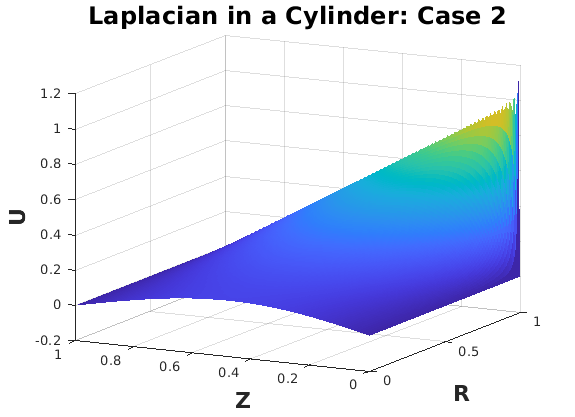
\includegraphics{lec32-ex2-plot-n150.png}
\caption{Solution for Case II with N=150.}
\label{fig:lec32-ex2-plot-n150}
\end{marginfigure}
The MATLAB code needed to construct this solution is shown in the listing below.
\begin{lstlisting}[style=myMatlab, name=lec32-ex2]
clear
clc
close 'all'

%% Case 2
R = 1; Z = 1;
g = @(z) 1-z; % temperature boundary condition
N = 150;

c = nan(N,1);
u = @(r,z) 0; % initialize the series
for n = 1:N
    c(n) = (1./besseli(0,n*pi)).*...
        integral(@(z) g(z).*sin(n*pi*z),0,Z)./...
        integral(@(z) sin(n*pi*z).*sin(n*pi*z),0,Z);
    
    % update the series with the next term
    u = @(r,z) u(r,z) + ...
        c(n)*besseli(0,n*pi*r).*sin(n*pi*z);
    
end

%% make surface plot
Rv = linspace(0,R,100);
Zv = linspace(0,Z,200);

[RR,ZZ] = meshgrid(Rv,Zv);
UU = u(RR,ZZ);

figure(1)
surf(Rv,Zv,UU,'edgecolor','none');
title('Laplacian in a Cylinder: Case 2',...
    'fontsize',18,'fontweight','bold');
xlabel('R','fontsize',16,'fontweight','bold');
ylabel('Z','fontsize',16,'fontweight','bold');
zlabel('U','fontsize',16,'fontweight','bold');
view([-63 15]);
\end{lstlisting}
